\section{Integración de la no holonomía}
\setlength{\columnseprule}{0pt}
\twocolumn
\subsection{Error de coordenadas polares}
Error de la meta con respecto al estado actual \cite{ramirez2001control}:
\begin{equation*}
    \mathbf{z}(t) = \begin{bmatrix} a \\ \alpha \end{bmatrix}
\end{equation*}
\subsection{Ley de control}
\vspace{-0.5cm}
\setlength{\overfullrule}{0pt}
\begin{equation*}
    \mathbf{u_{ref}} =
    \begin{bmatrix} v \\ \omega \end{bmatrix} =
    \begin{bmatrix}
        k_1\, a \cos\alpha \\
        k_2\,\alpha + k_1 \sin\alpha \cos\alpha
    \end{bmatrix}
\end{equation*}

% Mismo reveal que la diapositiva anterior: comparte el número de figura.
\addtocounter{figure}{-1}
\begin{figure}[H]
    \centering
    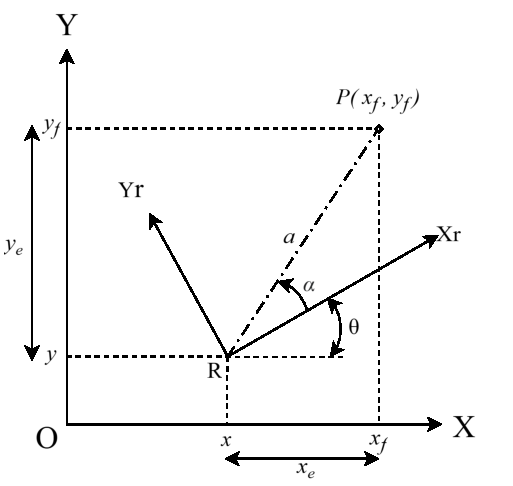
\includegraphics[width=0.9\linewidth]{Pics/error_construccion.pdf}
    \caption{Definición del error}
    \label{fig:error_control_polar}
\end{figure}
